\chapter{Basics of Neural Networks} \label{ch:neuronalNetwork}
Neural networks are networks of neurons in the mammalian brain \cite{ann}. A neuron consists of a cell body, dendrites and an axon which make it able to receive, process and send electric signals to other neurons and body cells. Through connection of these neurons, a brain can process information as we can experience in through our life. Humans have a proportionally big brain predicted to have around 86 billions neurons \cite{neurons}. Our brain gives us the level of intelligence enough to proceed with the complex functions of life and to 'think'. This ability has also inspired many scientists to develop a computational network with such potential of learning: an artificial neural network. 

%ANN
\section{Artificial Neural Network} \label{sec:ann}
First attempt to build such a network inspired by neural networks of the brain traced back to McCulloch and Pitts \cite{McandPitts}. Similarly, an artificial neuron receives many inputs and process an output which in turn becomes an input for other neurons on the further level. The simplest form with only a single neuron is a perceptron visualized in figure \ref{fig:perceptron}. The function of the perceptron will be discussed in detail in section \ref{perceptron}. In its simplest form, a neuron has weights it applies on the inputs. A neuron can be either active or inactive which is defined by whether the output exceeds a threshold or not. 


An artificial neural network (ANN) has many layers containing such neurons. The first layer is called the input layer where input data e.g. images is fed into and the last layer is the output layer, where the final output e.g. class prediction is sent as an answer of the system to the input. Between the input and the output layer, there are several hidden layers which process and transform the data, extract features and make necessary calculations for the final prediction. The number of the hidden layers determines whether a neural network is shallow, with only one hidden layer, or deep, with two or more hidden layers. There are several different models of neural networks which have their strengths and weaknesses making them more or less suitable for different tasks. The natures of the models are determined, for instance, by its ability to process higher-dimensional data or to store information from the pasts. These abilities are the results of how the layers are built up and how the internal interactions of the layers are planned.

 First, we will start with the simplest structure of neural networks consisted of only a single neuron, the perceptron, which also represents the simplest unit of any neural network. Then, to better understand the architecture of the network we use for the experiments, other relevant artificial neural network structures will be discussed.

\subsection{Perceptron} \label{perceptron}
\begin{figure}[tbh]
  \centering
    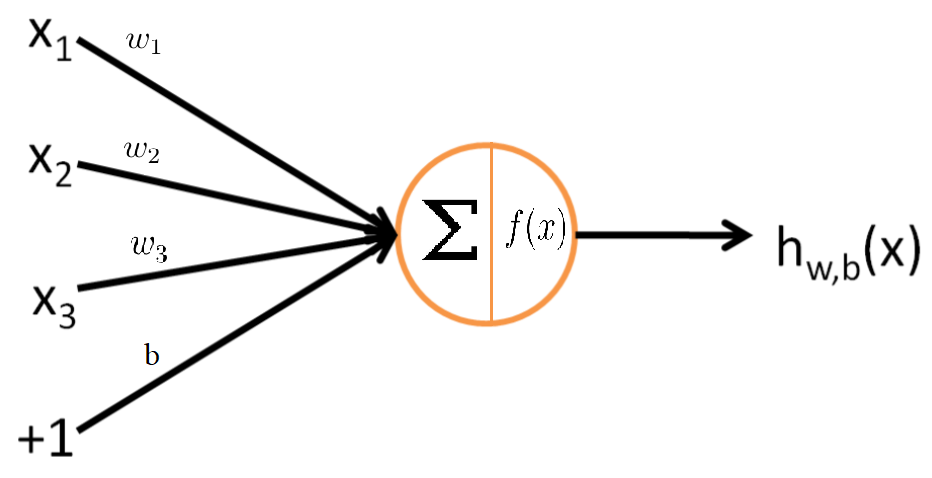
\includegraphics[width=0.5\linewidth]{abbildungen/perceptron.png}
  \caption{A perceptron: A perceptron contains a neuron and can take some inputs $\bm{x}$, applies weights $\bm{w}$ to them and generate an output $h_{w, b}(x)$. \cite{autoencoderSparse}}
\label{fig:perceptron}
\end{figure}

A perceptron is a neural network with only one neuron introduced by Frank Rosenblatt in \cite{perceptron}. The neuron in a perceptron has n inputs $x_1, x_2, ..., x_n$ which can be written as $\bm{x} = \left(x_1, x_2, x_3, \cdots, x_n \right)^T$ with an intercept input being +1, which is also called the bias term, the weights $w_1, w_2, ..., w_n$ applied to each input and an output $h_{w,b}(x)$ calculated by equation \eqref{eq:perceptronOut} with an activation function $f: \mathcal{R} \rightarrow \mathcal{R}$ indicating the behavior of the neuron. Examples for these functions are identity function \eqref{idFnc}, Heaviside function \eqref{heavisideFnc} and logistic function \eqref{logFnc}. The output behavior of the logistic function is shown in figure \ref{fig:logistic}. 
	\begin{equation} \label{eq:perceptronOut}
			h_{w,b}(x) = f(\bm{W^Tx}) = f(\overset{n}{\underset{i = 1}{\sum}}w_ix_i + b)
	\end{equation}
	\begin{equation} \label{idFnc}
			f(x) =  x
	\end{equation}
	\begin{equation} \label{heavisideFnc}
			f(x) =  H(x) = \left\{
		\begin{array}{ll} 
			0  & \mbox {, }x < 0 \\
			1 & \mbox {, }x  \leq 0
		\end{array}
	\right.
	\end{equation}
	\begin{equation} \label{logFnc}
			f(x) =  \frac{1}{1+e^{-x}}
	\end{equation}
	\begin{figure}[tbh]
  		\centering
    		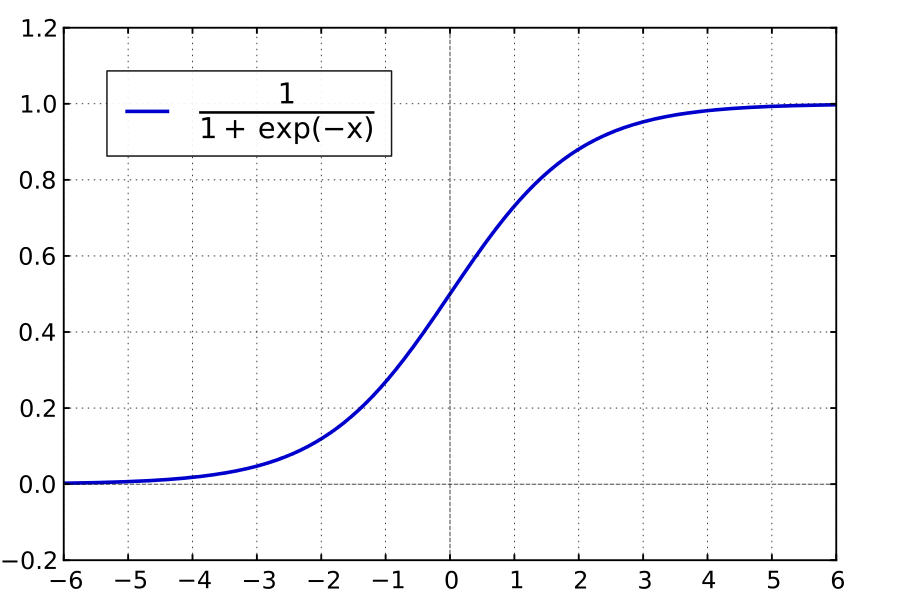
\includegraphics[width=0.8\linewidth]{abbildungen/logFnc.png}
  		\caption{Logistic Function: The value of the logistic function varies between 0 and 1 and can therefore represent the probability. The shape of the graph is also referred to as a Sigmoid curve.}  
		\label{fig:logistic}
		\end{figure}

The choice of the activation function must be made according to the task the network should handle. In case of a neuron with an all-or-nothing behavior, it is said to be active when the function value of $f$ exceeds a threshold, else it is inactive.

Since the effects of each inputs or each features on the output are controlled by the weights, the goal of training a neural network is to adjust the weights $w_i$ inside it so the output $h_{w, t}$ is as accurate as possible according to the task. For example, in a classification problem, the output of the well-trained network should correspond to the correct class of the objects it takes as an input. For this, choosing an activation function defining the output suitably for the task is crucial. In a linear regression problem where the output is linearly related to the input, a linear function might be more suitable and a function as step function that can be only 0 or 1 might be better for a binary classification with two competing classes. The higher the polynomial degree the activation function has, the finer the output can be tuned and accordingly, the more complex the task can be e.g. more possible classes the system can distinguish. On the other hand, if the chosen function is overly complex, it would cost more computing time than necessary for a simple task. 

The perceptron is only a neural network with only a single neuronal unit. The neural network commonly used in computer vision are consisted of many layers of neurons. To be able to understand the neural networks further, their learning processes should be understood. This includes how the knowledge is exchanged between each components and what is crucial to develop the right intelligence for the intended tasks. In the next section, the optimization of the networks with the common methods and possible mistakes are explained. 

%Network Optimization
\section{Network Optimization} \label{methods}
Before an ANN can perform the given task on its own, it must be trained first. By training an ANN, the weight of each neurons is adjusted so that it can generate the most accurate output for the desired prediction. As in figure \ref{fig:annSimp}, we will use the definitions from \cite{autoencoderSparse}, the output $\bm{a}_i^{l+1} = f(\bm{z}^{(l+1)})$ is the output from the activation function of the unit $i$ in layer $l+1$ computed from its input $\bm{z}^{(l+1)}$. Its weights $w_{ik}^{l+1}$ are assigned to its input $z^{l+1}_k$ and its bias term $b_i$. For the first layer $L_1$, the input layer, its input is $z^{(1)}_k = x_k$, the original inputs enter the first layer. For demonstration, the entering input $z^{(2)}$ and the forwarded output of the activation function of layer 2 with units $i \in \{1, 2, 3\}$ are:
	\begin{equation} \label{eq:act1L2} 
		a_1^{(2)} = f(w_{11}^{(1)}x_1 + w_{12}^{(1)}x_2 + w_{13}^{(1)}x_3 + b_1^{(1)})
	\end{equation} 
	\begin{equation} \label{eq:act2L2} 
		a_2^{(2)} = f(w_{21}^{(1)}x_1 + w_{22}^{(1)}x_2 + w_{23}^{(1)}x_3 + b_2^{(1)})
	\end{equation} 
	\begin{equation} \label{eq:act3L2} 
		a_3^{(2)} = f(w_{31}^{(1)}x_1 + w_{32}^{(1)}x_2 + w_{33}^{(1)}x_3 + b_3^{(1)})
	\end{equation} 

Then, these outputs from the second layer, the hidden layer, are assigned weights $w_{ik}^{2}$ and used to calculate the output of the final layer, the output layer $L_3$, which is also the output of this shallow neural network: 

	\begin{equation} \label{eq:output3ANN} 
		h_{w, b}(x) = a_1^{(3)} = f(w_{11}^{(2)}a_1 + w_{12}^{(2)}a_2 + w_{13}^{(2)}x_3 + b_1^{(2)})
	\end{equation} 

We can see that the outputs of each layer can be calculated consecutively from the former layers - from the beginning to the end only in the forward direction. A neural network with this behavior is also referred to as a feedforward neural network. Generally put, the outputs and inputs of the layers can be defined with following equations.
	\begin{equation} \label{eq:outputsANN} 
		\bm{z}^{(l+1)} = \bm{w}^{(l)}\bm{a}^{(l)} + \bm{b}^{(l)}
		\bm{a}^{(l+1)} = f(\bm{z}^{(l+1)})
	\end{equation} 

With this kind of networks, an effective strategy to adjust the weights according to the outputs is to trace the relations of the outputs from the outer layer back to the inputs and weights of the previous layers - to trace the outputs backwards into the hidden layers of the neural network. This method is also called the backpropagation algorithm \cite{backprop1986}. 

\begin{figure}[tbh]
  \centering
    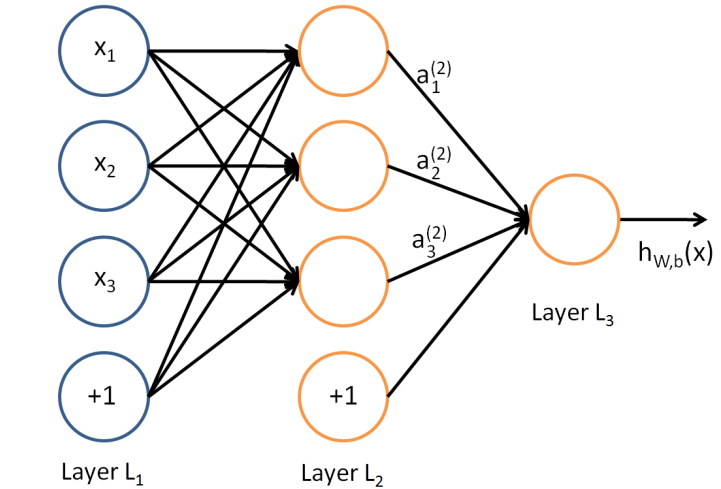
\includegraphics[width=0.5\linewidth]{abbildungen/annSimp.png}
  \caption{A simple ANN with a single hidden layer \cite{autoencoderSparse} An ANN takes the inputs through the neurons in the input layer $L_1$, then the weighted inputs are passed forward to the hidden layer $L_2$. The hidden layer then apply the activation function on the total inputs from the first layer and pass the calculated outputs $a_i^2$ to the output layer $L_3$. Finally, the output of the output layer $h_{w,b}$ is returned as the result.}
  \label{fig:annSimp}
\end{figure}

\subsection*{Backpropagation} \label{sec:backGD}
A simple ANN as shown  in figure \ref{fig:annSimp} might be sufficient for a simple problem. With more complex input data e.g. images or audio, a more complex network is needed to be able to learn the structure of the data sufficiently. As an ANN ‘learns’, it adjusts the weights of each neuron in its layers which can quickly sum up to millions of neurons. The goal of the adjustment is to find a combination of the weights that leads to the most accurate prediction of the data. With this kind of complexity, it is not wise to just blindly change the parameters until we get lucky and find the right ones. Therefore, the questions are how these million parameters can be adjusted efficiently and which direction of the adjustment is the right one.

The first question can be answered by the backpropagation algorithm. This algorithm is created to generalize the learning procedure of a perceptron, a single layer neural network, to multiple layer neural networks \cite{backpropagation} and became popular among researchers after the publication of \cite{backprop1986}. The main idea of backpropagation is to trace back into the hidden layers to adjust the weights of each layer accordingly so as to reduce the differences between the produced output and the desired ones. 

For simplicity, the derivation of this algorithm will not be explained in this thesis. The general theory of the backpropagation algorithm is explained extensively in \cite{backpropagation}.

Since our goal for a classification task is now to minimize the error of the prediction according to the labels of the data, the second question has to be brought back. To find the correct direction of the weight adjustment to achieve our goal, we can use gradient descent to ‘climb down the hill’ of the cost function until we reach the valley, the minimum point as illustrated in figure \ref{fig:GD}. In the next section, variations and functions of this algorithm will be described in details \cite{overviewGD}

\begin{figure}[tbh]
  \centering
    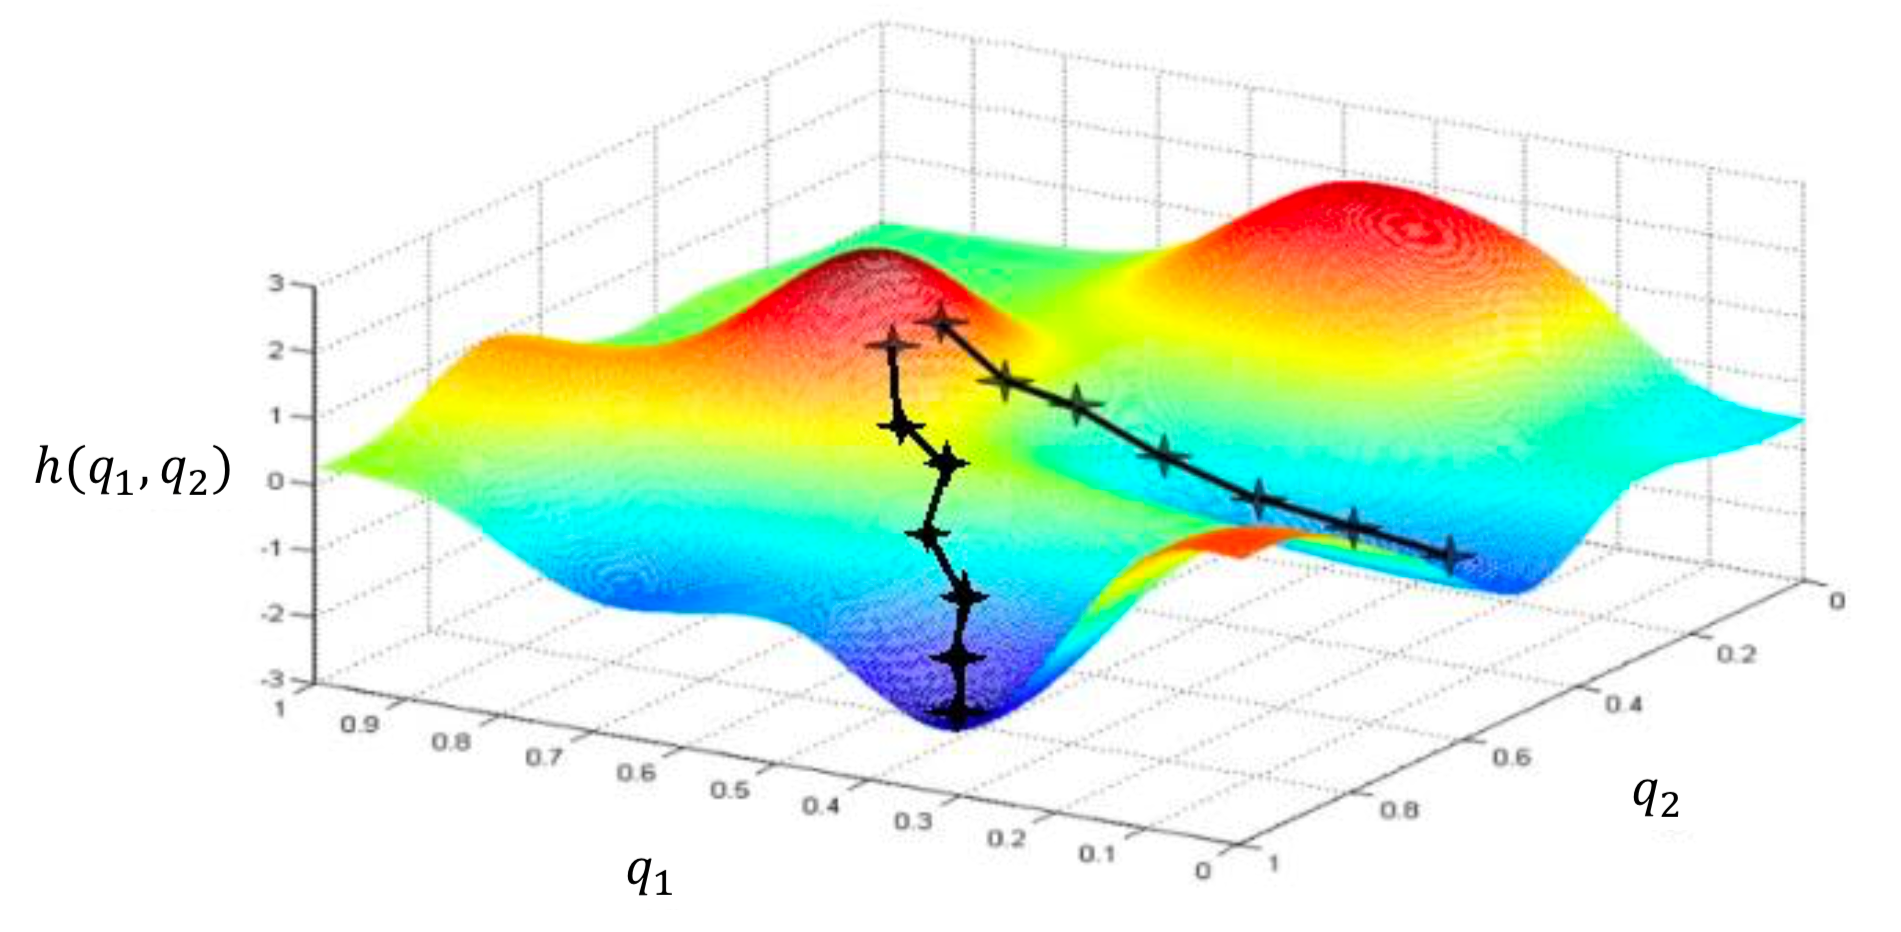
\includegraphics[width=\textwidth]{abbildungen/GD.png}
  \caption{Finding the minimum with gradient descent \cite{fig:GD}: With gradient descent, we try to minimize cost function $h(q_1, q_2)$ according to the parameters $q_1$ and $q_2$. As shown in the figure, it is also possible that we will find another local minimum if we chose another start point as the right start point takes us on the right route, the left point might take us on another route and to another local point. Therefore, initial parameters also influence the performance of the network.} 
  \label{fig:GD}
\end{figure}

\subsection*{Gradient Descent} \label{GD} 
The goal of training a neural network on a classification task is to find the parameter set with which it can make the most accurate prediction according to the input. In order to do this, we define a cost function of the network gets higher if the prediction is far from the reality, a function that measures the error of the network. Therefore, we can say that our goal is to minimize the value of the cost function - to find the parameter set that takes as to this point. The most effective way to do this is to always step in the direction that goes down the steepest. The steepness or the amount of change in a function over its parameters can be measured by its derivative $\frac{dJ}{d\theta_i}$ over its parameter $\theta_i$.  From the computed derivative, we know in which direction the strongest positive slope, the gradient, goes and make a step in the opposite direction - hence, gradient descent. The size of the step we take depends on the learning rate $\lambda$. Iteratively, we calculate the derivative and take a step until we reach the local minimum point of the cost function. 

An example of possible cost functions is the sum of squared errors $E_{sse}$ \eqref{eq:sseFnc} which sums up squared errors between a set of values. This can be used to measure how far off the $n$ predicted values $h_{w, b}(x_k)$ from the network are from the ground-truth values $y_k$.
	\begin{equation} \label{eq:sseFnc} 
		E_{sse} = \frac{1}{2}\overset{n}{\underset{i = 1}{\sum}}(h_{\bm{w},\bm{b}}(x_k) - y_k)^2
	\end{equation} 


The bigger the sum of the errors is, the more often and the bigger the differences were made. To make better predictions, the network should learn to reduce this sum - it should be optimized to minimize this error. According to equation \ref{eq:outputsANN}, the final output of the network $h_{w, b}(x_k)$ is a function of the weights $w_{ik}^{(l)}$ and the biases $b_i^l$. This means that the loss $E_{sse}$ is also parameterized by these values and adjusting them correctly can reduce the amount of error. The key to optimize the loss is to change the weights. Mathematically, a change of a function over a parameter is its derivative over the parameter. The change over a specific parameter, in particular, is represented by the partial derivative of this parameter. Gradient descent works by computing the change in the loss function caused by changes in the weights, i.e., the partial derivatives of the loss function over each weight $ \frac{\partial E_{sse}(\bm{w}, \bm{b})}{\partial w_{ik}^(l)}$ After the calculation, the weights and the biases are updated after \eqref{eq:weightUpdate} and \eqref{eq:biasUpdate}with the learning rate $\lambda$ controlling how big the adjustment after a round of backpropagation should be.

	\begin{equation} \label{eq:weightUpdate} 
		w_{ij}^{(l)} = w_{ij}^{(l)} - \lambda \frac{\partial}{\partial w_{ij}^{(l)}}E_{sse}(\bm{w}, \bm{b})
	\end{equation} 
	\begin{equation} \label{eq:biasUpdate} 
		b_{i}^{(l)} = b_{i}^{(l)} - \lambda \frac{\partial}{\partial b_{i}^{(l)}}E_{sse}(\bm{w}, \bm{b})
	\end{equation} 


The gradient descent algorithms need the input data to calculate the gradients. There are several variations of how much data we want to use for the calculations and which algorithms we use to calculate the gradient. First, the variation on the data amount will be introduced. This section is based on \cite{overviewGD}.

\subsubsection*{I Variations of Gradient Descent}
The amount of input data used for the calculation of the gradient has an impact on the accuracy of the computation. The more input data is used, the more accurate the value will be but also the longer the computation will take. By changing the amount of data, we can tweak the balance between the speed and the accuracy of the calculation. There are three common ways to do this: use the entire training dataset, use only one sample at a time, or take a sample batch from the dataset. 

\paragraph*{i) Batch Gradient Descent} Batch gradient descent uses the whole training dataset to calculate the gradients for each step. This makes it comparatively slow, memory-expensive and incompatible for updating gradient online with new examples coming in. However, since there is no fluctuation between the data for each calculation, it surely finds a minimum according to the initial parameters it started from, the global one for convex surfaces and a local minimum for non-convex surfaces. An example of these surfaces is visualized in figure \ref{fig:convex}. With this variation, we prioritize the accuracy more than time.  

\begin{figure}[tbh]
  \centering
    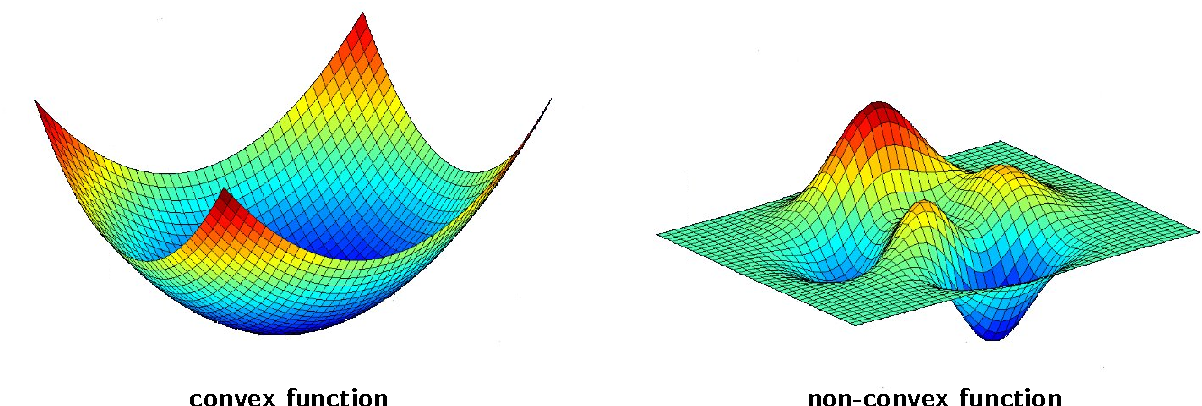
\includegraphics[width=0.8\textwidth]{abbildungen/convex.png}
  \caption{Convex and non-convex functions: A convex function has only a single minimum. A non-convex function, in contrary, has several local minima with a global minimum, the lowest minimum.} 
  \label{fig:convex}
\end{figure}

\paragraph*{ii) Stochastic Gradient Descent} \label{stochGD}This variation of gradient descent makes the opposite trade-off to the batch gradient descent by randomly taking just one training sample for each gradient calculation. Therefore, it takes much less time to calculate and update parameters which is more suitable for training online. Since there is variance between each step, the fluctuation can cause overshooting when converging to a minimum. While this can affect the path to the exact minimum, it also allows finding a better local minimum by springing out of the valley in which it started. Furthermore, there is a solution to the overshooting problem: a slowly decreasing learning rate has been shown to help SGD to convert to an exact minimum as the batch gradient descent \cite{overviewGD}. 

\paragraph*{iii) Mini-batch Gradient Descent} The small-batch gradient descent is the most popular variation of the gradient descent algorithm for training a neural network. It is practically in the middle of the former two variations as the gradient is calculated by using a batch of samples from the training dataset - not all of the dataset and not just a single sample. By doing this, there is less fluctuation between each parameter updates which means a more stable convergence. In the experiments in this thesis, this method is used with a batch size of 32 samples each iteration.

Apart from changing the amount of data used for the gradient calculation, we also can use an optimization method to counter different challenges in the process of finding the right parameters. Now, two examples of available optimization will be described.

\subsubsection*{II Optimization algorithms for Gradient Descent}
\paragraph*{i) Momentum} The momentum method \cite{momentum} is used to counter the problem of oscillating path caused by unevenly steep slopes in directions of different parameters. This is also found when the features significantly vary in their values. An illustration of such problem is shown in figure \ref{fig:ovalPlane}. This method adds a part of the past update vector to the recent one creating an acceleration along the way to the valley. The parameter is updated after equation \eqref{momentumFnc} and \eqref{momentumthetaFnc}.

	\begin{equation} \label{momentumFnc}
			v_t = \gamma v_{t-1} + {\eta}{\bigtriangledown_\theta}E(\theta)
	\end{equation}

	\begin{equation} \label{momentumthetaFnc}
			\theta = \theta - v_t
	\end{equation}

with an update vector $v_t$ at step $t$, a cost function $E$ and the parameter that should be update $\theta$.

This original momentum algorithm uses the recent position of the parameters to perform the update of the parameter. Therefore, it has no insight of the next step and could make a sub-optimal adjustment. Next, an algorithm is introduced that uses the information from the future position of the parameters.
 
\begin{figure}[tbh]
  \centering
    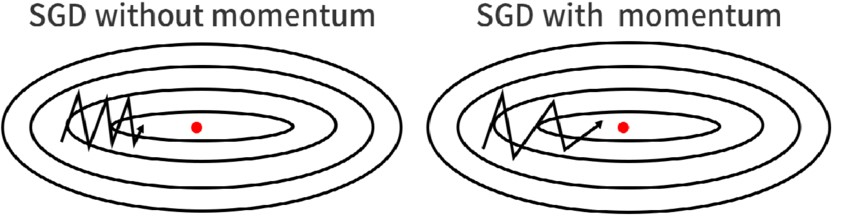
\includegraphics[width=\textwidth]{abbildungen/momentumGD.jpg}
  \caption{Stochastic Gradient Descent with and without momentum \cite{fig:momentumGD}: Without the momentum optimization, the path of the gradient descent suffers from the oscillation when the features are of different multitudes as can be seen in the left picture. The momentum accumulated in the direction of the longer axis allows for a more direct descending path as depicted on the right.} 
  \label{fig:ovalPlane}
\end{figure}

\paragraph*{ii) Nescerov Accelerated Gradient (NAG) \cite{NAG}} This algorithm is the speed-up version of the momentum. Instead of using the present parameter position to calculate the gradient, it approximately calculates the gradient of the slope in the next step. This way, it adapts to the next position and looks ahead down the hill instead of just adjusting itself to the hill as it descends. According to equation \eqref{eq:nescerovFnc}, this algorithm calculates the gradient using $\theta - \gamma v_{t-1}$, the approximated of the future $\theta$, instead of just $\theta$, to calculate the vector. Then, it similarly updates the parameter using the calculated vector \eqref{eq:thetanescerovFnc}.

	\begin{equation} \label{eq:nescerovFnc}
			v_t = \gamma v_{t-1} + {\eta}{\bigtriangledown_\theta}E(\theta - \gamma v_{t-1}) 
	\end{equation}
	\begin{equation} \label{eq:thetanescerovFnc}
			\theta = \theta - v_t
	\end{equation}

\paragraph*{iv) Adaptive Moment Estimation (Adam)} Adam \cite{adam} is an adaptive learning method, i.e. it computes learning rates for each parameter individually. With an adaptive method like this, the size of the update for a parameter is smaller, the more frequent this parameter is updated. As its name implies, Adam also uses moments to calculate the updates as following: first, it calculates and collects the decaying moment according to equation \eqref{eq:AdammomentFnc} with the decay rates $\beta_1$ and $\beta_2$. Then, it corrects their bias towards 0 caused by initialized values $m_v$ and $t_v$ being 0, according to \eqref{eq:AdamcorrectFnc}. 

	\begin{equation} \label{eq:AdammomentFnc}
		\begin{split}
			g_t = & {\bigtriangledown_{\theta_t}}J(\theta_t) \\
			m_t = \beta_1m_{t - 1} &+ (1 - \beta_1)g_t \\
			v_t = \beta_2v_{t - 1} &+ (1 - \beta_2)g^2_t
			\end{split}
	\end{equation}

	\begin{equation} \label{eq:AdamcorrectFnc}
	\begin{split}
		\hat{m}_t = \frac{m_t}{1 - \beta_1^t} \\
		\hat{v}_t = \frac{v_t}{1 - \beta_2^t}
	\end{split}
	\end{equation}

Finally the parameters are updated with help of the calculated moments as defined in equation \eqref{eq:AdamupdateFnc}

	\begin{equation} \label{eq:AdamupdateFnc}
			\theta_{t+1} = \theta_t - \frac{\eta}{\sqrt{\hat{v}_t} + \epsilon} \hat{m}_t 
	\end{equation}

\paragraph*{Nesterov-accelerated Adaptive Moment Estimation (Nadam)} As the name implies, this algorithm is the combination of the previous two methods, the Nescerov accelerated gradient and Adam. This gives us the new parameter updating rule \eqref{eq:nadamupdateFnc} 
	\begin{equation} \label{eq:nadamupdateFnc}
			\theta_{t+1} = \theta_t - \frac{\eta}{\sqrt{\hat{v}_t} + \epsilon} \left( \beta_1\hat{m}_t + \frac{(1 - \beta_1)g_t}{1 - \beta_1^t} \right)
	\end{equation}
With this method, the gradient descent is accelerated and adapts well to both the curve of the cost function and different parameters at the same time.

After we addressed the method of training the network effectively using backpropagation and gradient descent. We will now introduce of the common perils in the training that can affect the performance of the network.

\subsection{Overfitting and Underfitting}
When training a neural network, choosing the right method to the problem and the given data is important to ensure that the network will learn the information necessary for the task. Then, choosing the right parameters so that the training goes as plan is also crucial. All these correct setups could only be optimal if we know what danger still awaits in the training which can compromise the performance of the model. The common problems occuring in the training are overfitting and underfitting. Overfitting is when the network adapts itself too much to the data and underfitting is when the network could not or would not adapt enough to learn the problem. More details and prevention methods to these problems are discussed now in this section. 
 
\subsection*{A. Overfitting}
Overfitting describes a situation when a model starts to learn unnecessary noises and irregularities in the training set and not the more relevant knowledge it should for the task. In the end, the network would not generalize well on new data because it has adapted itself too much on the training dataset. Similar to a student memorizing the answers to the exercise sheets but has no real knowledge about the underlying theories in the subject, the network will know the training data very well but will not perform well on the unknown data, the real test. The problem of overfitting is visualized in figure \ref{fig:underoverfitting} along with underfitting. The overfitted curve adjusts itself to each and every data point it has seen in the training. Consequently, it has overall an inaccurate representation of the true distribution even if the error calculated on the given training data is very low. Since the main goal of training the networks is not only to learn specifically about the training data, but to have enough general knowledge to perform the task on the unknown data, overfitting can compromise the performance of the trained networks.

Overfitting can happen especially when the model is complex enough and is trained repeatedly too much on the same data, e.g. too many epochs have passed or too little data for the complexity of the networks. We should suspect a problem of overfitting when the model has a good performance or a very low loss value in the training data but has a low performance on other data. Note that this symptoms might also come from other underlying causes. 

\paragraph*{Prevention of Overfitting}
To prevent overfitting, we have to avoid over-training the models i.e. training further even if the model has reached the convergence of the loss function. Even an experience researcher cannot be certain of the point at which the training should be terminated. Therefore, more exact ways to automatically achieve this was developed. Here, two examples of such possibilities are listed: early stopping and training with weight decay.  

\subparagraph*{i. Early stopping} Ideally, we should stop training early enough so that the model has already learned to fit its function to the nature of the data seen in the training but not enough to overly fit it exclusively to this data. To know when to stop needs much experience and can also cost an unnecessary performance drop if not done right, therefore using an algorithm to automatically stop the training is introduced. For this, the training set is divided into an actual training set and a validation set with a proportion of 2 to 1 \cite{overfitearlystop}, then to observe the loss on the validation set after training e.g. for an epoch. An example for a stop criterion: if the validation loss increase relatively high after an epoch, the training is then stopped. Formally, after epoch $t$, we have the validation loss $E_{va}(t)$ defined by a loss function for training and the lowest validation error so far in the training $E_{opt}(t) = \underset{t'\leq t}{min}E_{va}(t')$. We can define the generalization loss $GL(t)$ as the relative increase of the validation error over the recorded minimum as in \eqref{eq:earlystop}. If the generalization loss exceeds a threshold, the training should stop. 
	\begin{equation} \label{eq:earlystop}
			GL(t) = 100 \left( \frac{E_{va}(t)}{E_{opt}(t)} - 1 \right)
	\end{equation}
This algorithm stops training automatically when the risk of overfitting appears at a cost of extra training time. \cite{overfitearlystop} shows different setup and the tradeoff between time and performance increase. 
\subparagraph*{ii. Weigth Decay} Another possibility to prevent overfitting is to penalize big weights in the network. As we saw in $\ref{perceptron}$, each neuron has its weights to adjust the influence of the input on the output. With weight decay, the original loss function $E_0(\bm{w})$ is combined with the weight penalizing term into a new cost function as follow: 	
	\begin{equation} \label{eq:weightdecay}
			E(\bm{w}) = E_0(\bm{w}) + \frac{1}{2}\lambda\underset{i}{\sum}\bm{w}_i^2
	\end{equation}
where $\lambda$ is the learning rate and $\bm{w}$ the weights of the neurons. 

By penalizing the weights, we put constraints on the network and limit its freedom to adjust the parameters freely. This prevents the weights from growing unnecessary large and was proved to improve the generalization of the network \cite{overfitweightdecay}. It is also a preferable alternative to eliminating the number of weight to keep the network as simple as possible as proposed in \cite{overfitweightelim}.

\subsection*{B. Underfitting}
The problem of underfitting is the opposite of the overfitting case \cite{underoverfitting}. It happens when the network is not complex enough to learn the underlying nature of the problem. For example, if we want to find a fit for non-linearly distributed data a linear model, the model cannot be adjusted enough to describe the problem accurately. To avoid this, the choosing a network with proper complexity to the problem is crucial. The choice must also take into account the amount of data we have to also avoid overfitting at the same time. 

\begin{figure}[tbh]
  \centering
    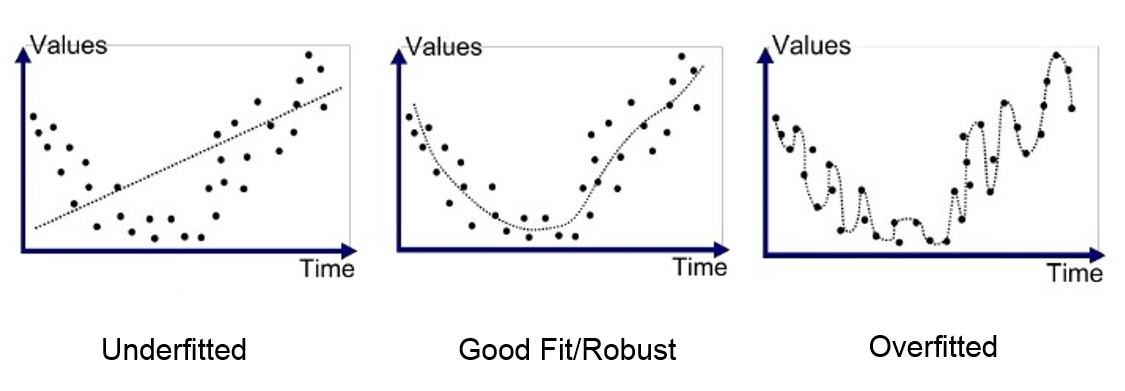
\includegraphics[width=\textwidth]{abbildungen/overunderfitting.png}
  \caption{Overfitting and Underfitting: A good representation of the underlying distribution of the given data points is depicted in the middle. The underfitted representation has insufficient dimensionality to represent the real distribution as shown in the left graph. If the network has overfitted itself, as on the right, it tries to adjust itself to every given point and thus would mostly make poor predictions on unknown data points.} 
  \label{fig:underoverfitting}
\end{figure}

As the neural network becomes more complicated with more neurons and more layers, the relation between the output, the weights and the inputs become more complex and can handle more difficult tasks effectively as a perceptron cannot. To handle such inputs as images or audio files, a network of higher complexity is necessary for effective task handling. In computer vision, one type of neural networks in particular has become very popular and is also included in the Domain Separation Network we use here. Therefore, the structure of this neural network, the Convolutional Neural Network, will be explained more in detail in section \ref{cnn}.


%CNN
\subsection{Convolutional Neural Network} \label{cnn}
The goal of computer vision is to make machines see as we can with our eyes and brains. Intuitively, we identify object with noticeable high-level features such as body composition of an animal or part of an object. For a machine to be able to do this, it requires building up detectable low-level features together until they represent a part. Dots build up lines, lines join to create edges and edges define forms of a part of an object that hints to an object. A CNN is built of many stages extracting different features on different levels to put them back together and make prediction about the image as a whole.  Each stage consists of layers of neurons which are described further in this section. The definition of the structure is based on \cite{convVision}.

\paragraph*{Common Layers of the Convolutional Neural Networks}
\subparagraph*{i. Filter Bank Layer or Convolutional Layer} In this layer, different features in an input image are detected by different filters. Each filter has weights with a filter-specific kernel to 
convolve with the feature maps as described in Equation \ref{fig:conv} and each neuron has its receptive field or an area of image it scans for the feature. Because all areas of the images get scanned with the filters thoroughly, the features are detected even if their position changes. This process is visualized in figure \ref{fig:conv} Mathematically described, the 3D input array consists of $n$ 2D images $x_i$. The filter kernel $k_{ij}$maps the input $x_i$ to the feature map $y_j$ as an output according to equation \eqref{convFnc} where $\ast$ is the 2D discrete convolution operator defined as \eqref{convOpFnc}
\begin{equation} \label{convFnc}
			y_i = b_j + {\sum_i}k_{ij} \ast x_i
\end{equation} 
\begin{equation} \label{convOpFnc}
			h \ast x = \overset{\infty}{\underset{k_1 = -\infty}{\sum}}\overset{\infty}{\underset{k_2 = -\infty}{\sum}} \cdots \overset{\infty}{\underset{k_M = -\infty}{\sum}} h(k_1, k_2, \cdots, k_M) x(n_1 - k_1, n_2 - k_2, \cdots, n_M - k_M)
\end{equation}

The size of the output of the $n$-th layer $(M_1^n, M_2^n)$ will depend on the size of the input, the output from the $(n-1)$-th layer, $(M_1^{n-1}, M_2^{n-1})$ and the size of the kernel $(K_1^n, K_2^n)$ with a stride of size $(S_1^n, S_2^n)$ as follow \cite{flexHighCNN}:
\begin{equation}
			M_1^n = \frac{\left(M_1^{n-1} - K_1^n\right)}{S_1^n + 1} + 1 
\end{equation}
\begin{equation}
			M_2^n = \frac{\left(M_2^{n-1} - K_2^n\right)}{S_2^n + 1} + 1 
\end{equation}

As we can see from figure \ref{fig:conv} and the equations above, the feature map will be smaller after the convolution. To control the size change, padding can be used to extend the input around the edges. A typical padding variation is to extend the edges with zeros. The size of the output of the $n$-th layer $(M_1^n, M_2^n)$ will depend on the size of the input, the output from the $(n-1)$-th layer, $(M_1^{n-1}, M_2^{n-1})$ and the size of the kernel $(K_1^n, K_2^n)$ with a stride of size $(S_1^n, S_2^n)$ and $p$ zero padding size as follow \cite{convArith}:
\begin{equation}
			M_1^n = \frac{\left(M_1^{n-1} - K_1^n + 2p\right)}{S_1^n} + 1 
\end{equation}
\begin{equation}
			M_2^n = \frac{\left(M_2^{n-1} - K_2^n  + 2p\right)}{S_2^n + 1} + 1 
\end{equation}


\begin{figure}[tbh]
  \centering
    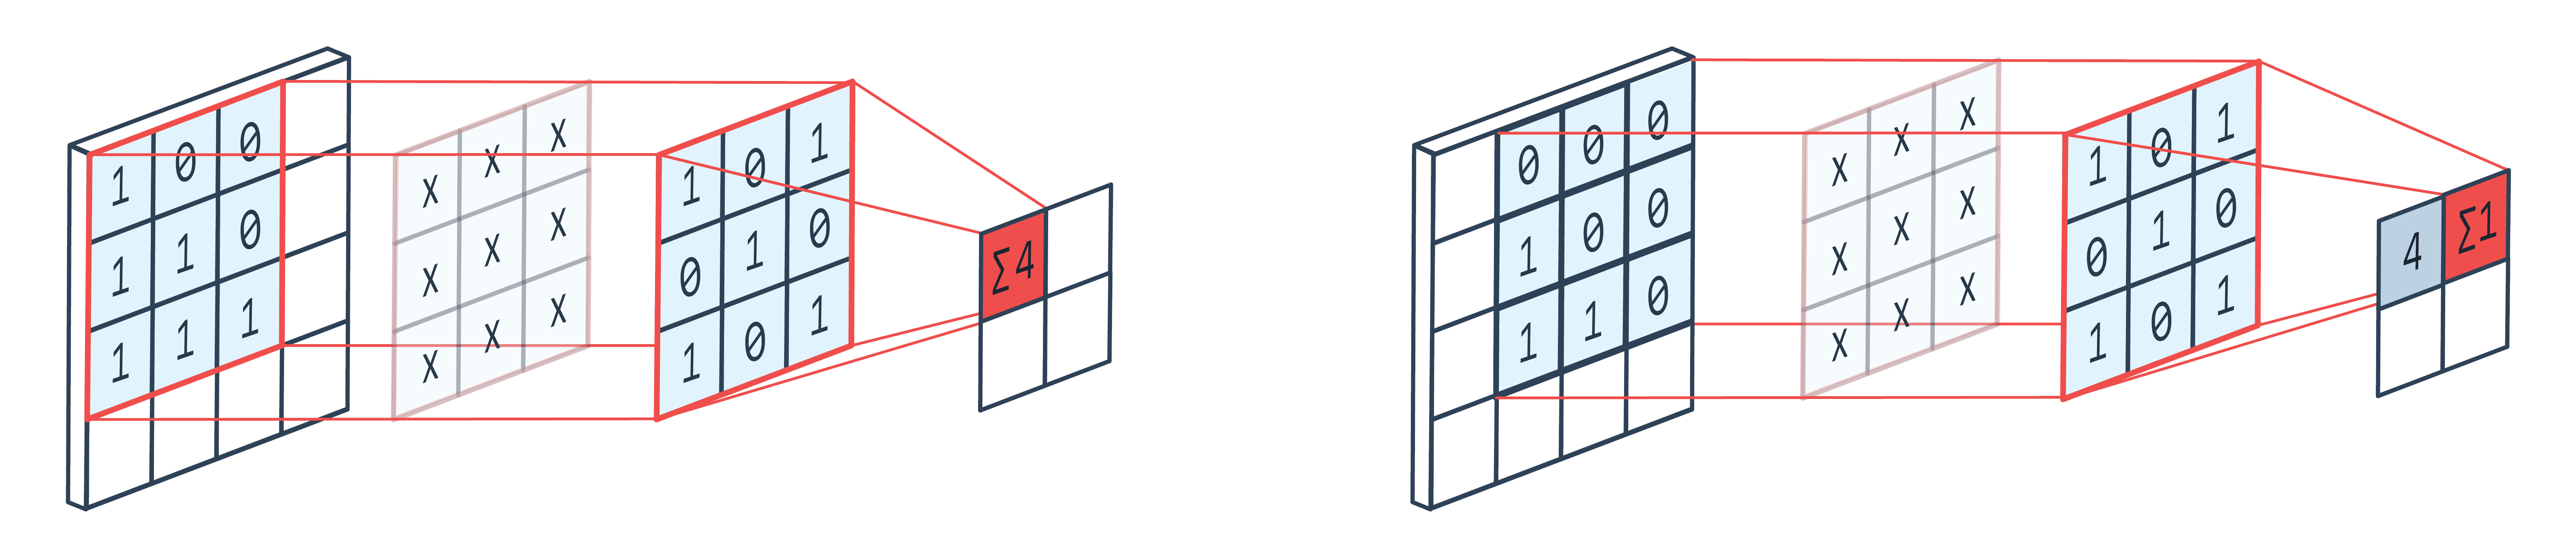
\includegraphics[width=\linewidth]{abbildungen/conv.png}
  \caption{Convolution with a 3x3 kernel \cite{fig:conv}: An 4x4 image is convolved with a 3x3 kernel. The kernel strides one pixel at a time and compute in each step a value for the output matrix. Since there is no padding, the dimension of the output is smaller than that of the input.} 
  \label{fig:conv} 
\end{figure}

\subparagraph*{ii. Non-linearity Layer}This layer hosts a nonlinear function used to compute the outputs of the neurons such as tanh function defined by equation \eqref{tanhFnc} or logistic function as defined in \eqref{logFnc}. In the method we use in this thesis, the rectified linear unit \cite{reluICML} defined by equation \eqref{reluFnc} is used which allows faster training than the $tanh$ function \cite{imgNet}. 
	\begin{equation} \label{tanhFnc}
			f(x) = \frac{e^x - e^{-x}}{e^x + e^{-x}}
	\end{equation}
	\begin{equation} \label{reluFnc}
			f(x) =  max(0, x)
	\end{equation}

\subparagraph*{iii. Pooling Layer:}This layer reduces the resolution of its input, the output of the previous layer, by computing a representative value such as the average value, using average pooling or the maximum value of a region in the input. Different outputs from these two methods can be seen in figure \ref{fig:pooling}. \cite{cnnpooling} has proved that using maximum value can achieve better performance. In the architecture we use, DSN also uses a model with max-pooling layers which samples out the maximum value to downsize the input and also makes its position invariant over bigger region \cite{flexHighCNN}.

\begin{figure}[tbh]
  \centering
    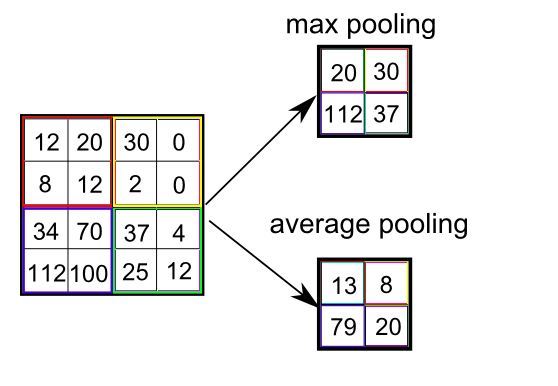
\includegraphics[width=0.6\linewidth]{abbildungen/pooling.png}
  \caption{Output of Max Pooling and Average Pooling \cite{fig:pooling}: From the same input matrix of dimension 4x4, a 2x2 pooling operation with a stride of 2 pixels gives an 2x2 matrix as an output with different value dependent from the method. The max pooling method pulls out the maximum value in each areas and the average pooling method calculates the average of the area. } 
  \label{fig:pooling} 
\end{figure}

A typical CNN contains two or three stages with these layers. Then, the outputs of various feature filters in the last stage are connected in the fully connected layer to compute final output in the desired form. For this purpose, it might get flattened into a one-dimensional vector. In our classification task, the probabilities of each classes are computed to be the final output. After all the stages, we get the output from the final output layer. An Example of a CNN with these layers are shown in figure \ref{fig:cnn}

\begin{figure}[tbh]
  \centering
    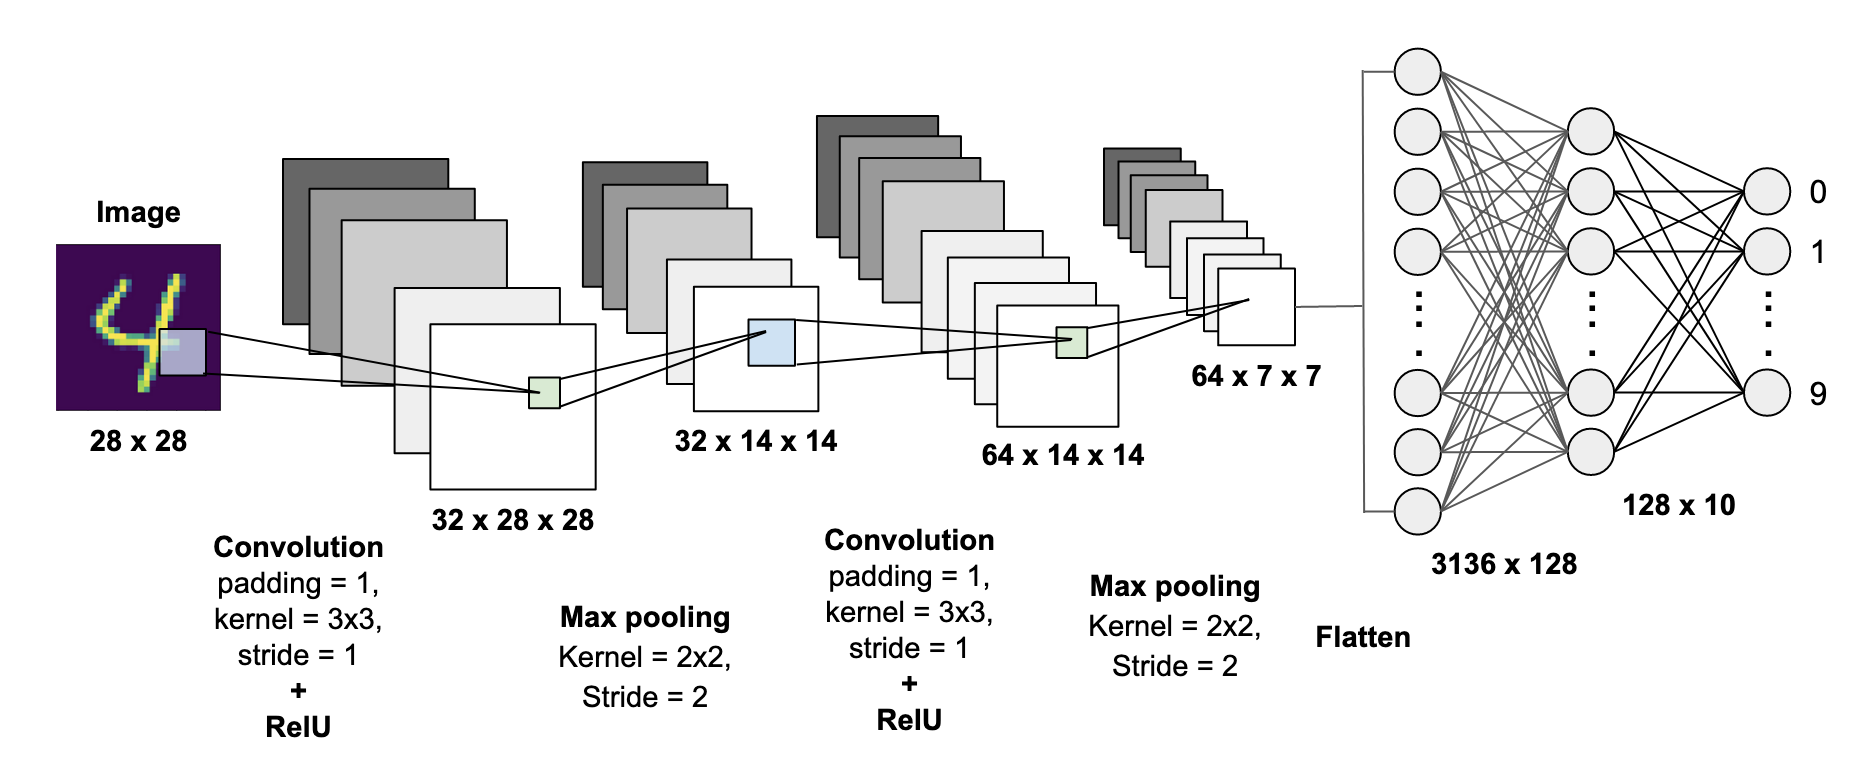
\includegraphics[width=\linewidth]{abbildungen/cnn.png}
  \caption{Convolutional Neural Network \cite{fig:cnn}: This CNN should recognize the number in the input image. It contains two stages with three layers: a convolutional layer, a non-linearity layer with ReLU, and a pooling layer. At the end, it should output the predictions on the class of the image being 0 to 9.} 
  \label{fig:cnn} 
\end{figure}

\paragraph*{Applications of the Convolutional Neural Networks}
The power of the deep convolutional neural networks are demonstrated in \cite{imgNet} as a team won the ImageNet Large Scale Visual Recognition Challenge 2012 \cite{ILSVRC2012} in both the classification and localization tasks with this kind of neural networks. Their deep CNN has 60 million parameters and 650,000 neurons with five convolutional layers followed partly by max-pooling layers and three fully connected layers. A way to effectively train this large network is through stochastic gradient descent method described in Section \ref{stochGD}.

Furthermore, the CNN was used, for example, to extract and transfer style of images in \cite{convImgStyle}. Through several convolutional layers, the features of the image styles are extracted and can be used to combine with another image to represent that image in the extracted style (see figure \ref{fig:styleTrans}). In this work, we can also see the different levels of extracted features from different layers in the CNN as shown in figure \ref{fig:cnnLevel}

\begin{figure}[tbh]
  \centering
    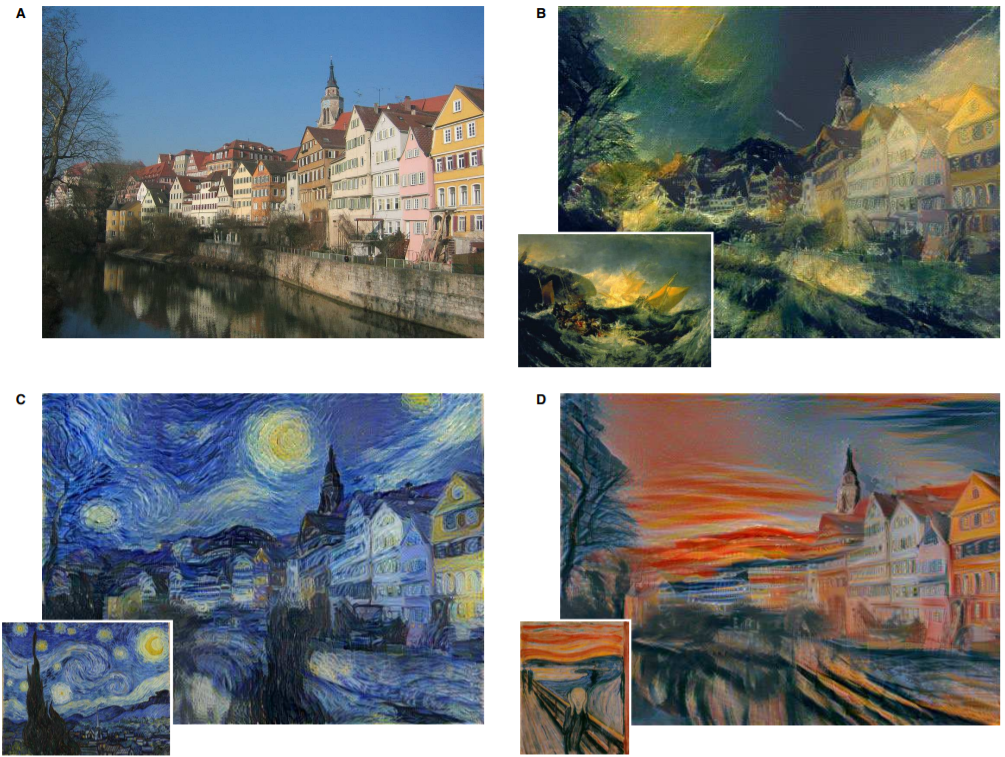
\includegraphics[width=\linewidth]{abbildungen/styleTrans.png}
  \caption{Style Transfer by a CNN: By extracting the style of famous pictures and the contents of the image, a CNN can produce the given image in the given styles \cite{convImgStyle}.} 
  \label{fig:styleTrans} 
\end{figure}

\begin{figure}[tbh]
  \centering
    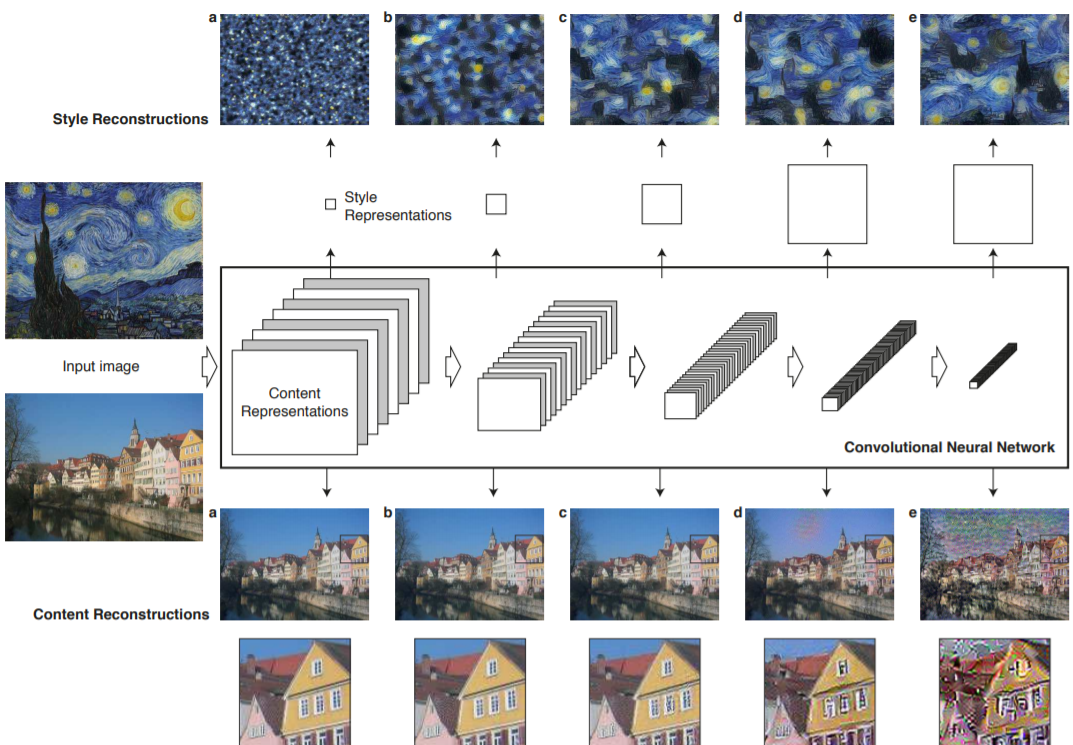
\includegraphics[width=\linewidth]{abbildungen/cnnLevel.png}
  \caption{Output from different levels in a CNN: Deeper levels of a CNN can capture more high-level details of the style and the components of the images whereas the first levels acquire the details finer on the pixel level.} 
  \label{fig:cnnLevel} 
\end{figure}


%Autoencoders
\subsection{Autoencoders} \label{sec:autoencoders}
When working with images, the common challenges are dealing with the dimensions of the image. The motivation for the autoencoders is to find lower-dimensional representations of a high-dimensional input from which the original input can be reconstructed. For example, images with higher solution can be represented by lower-dimensional features with the autoencoders. Furthermore, to be able to represent something with less details, its significant points must be preserved. This way, the autoencoders can also extract features and create representations that are more suitable for further tasks \cite{autoencoderVisualize}. 

\begin{figure}[tbh]
  \centering
    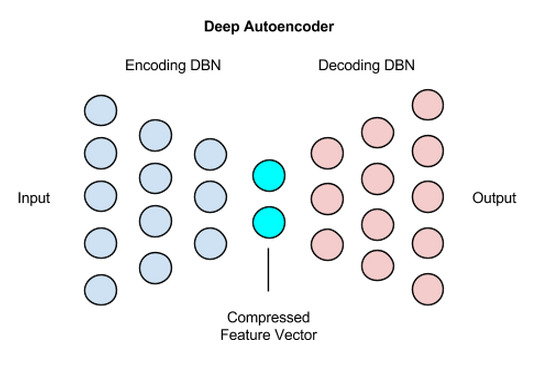
\includegraphics[width=0.6\linewidth]{abbildungen/autoencoders.png}
  \caption{Example of an autoencoder: The autoencoder encodes an input into a lower-dimensional feature vector. This representation can then be decoded back to higher-dimensional inputs as the original \cite{fig:autoencoders}.}
  \label{fig:autoencoders} 
\end{figure}

An autoencoder, therefore, has two essential parts: an encoder and a decoder. The encoder extracts the significant features of the input and maps these into a lower-dimensional output. The decoder then maps the encoded output, ideally, back to the original information. Formally, the encoder has a function that maps a $d$-dimensional input $x_i \in \bm{X}$ with a function $f$ a representation $\bm{h} = f(\bm{x}), h \in \bm{H}$ with dimension $p \ll d$. Note that it is possible to have an autoencoder with $p = p_1 + p_2 > d$ \cite{autoencoderDeep} which is not relevant in our case. Then, the decoder has a function $g$ that maps back the representation $h$ to a $d$-dimensional output. The mapping functions work in a way that:
 	\begin{equation} \label{eq:autoencoder}
			|x - (g \circ f)(x)| \rightarrow min
	\end{equation}

The representation the decoder maps from the encoded values $(g \circ f)(x)$ should be as similar to the original input $x$ as possible - the difference to the original input must be minimized. By trying to find lower-dimensional representations of the inputs and to decode these representations back to outputs resembling the original ones, the autoencoders find applications in many fields as feature extracting and dimension reduction are generally helpful to the working of neural networks. In the DSN, the autoencoders also extract representations used to apply domain adaptation and to train the classifier. 



\paragraph*{Applications of the Autoencoders} 
\subparagraph*{Dimensionality Reduction \cite{autoencoderVisualize}} The main benefit of the autoencoders is that they can find representations of the inputs with lower dimensions than the original input. An autoencoder can find codes for the images with 28x28 pixels from the MNIST dataset with only two dimensions that still show a clear separations of classes as visualized in figure \ref{fig:mnistvisualize}, even better than those created by the principle component analysis (PCA) \cite{PCA}, a method popularly used to extract features. The autoencoder can find representation for pictures of human faces with only 30 dimensions as shown by \cite{autoencoderFace}.

\begin{figure}[tbh]
  \centering
    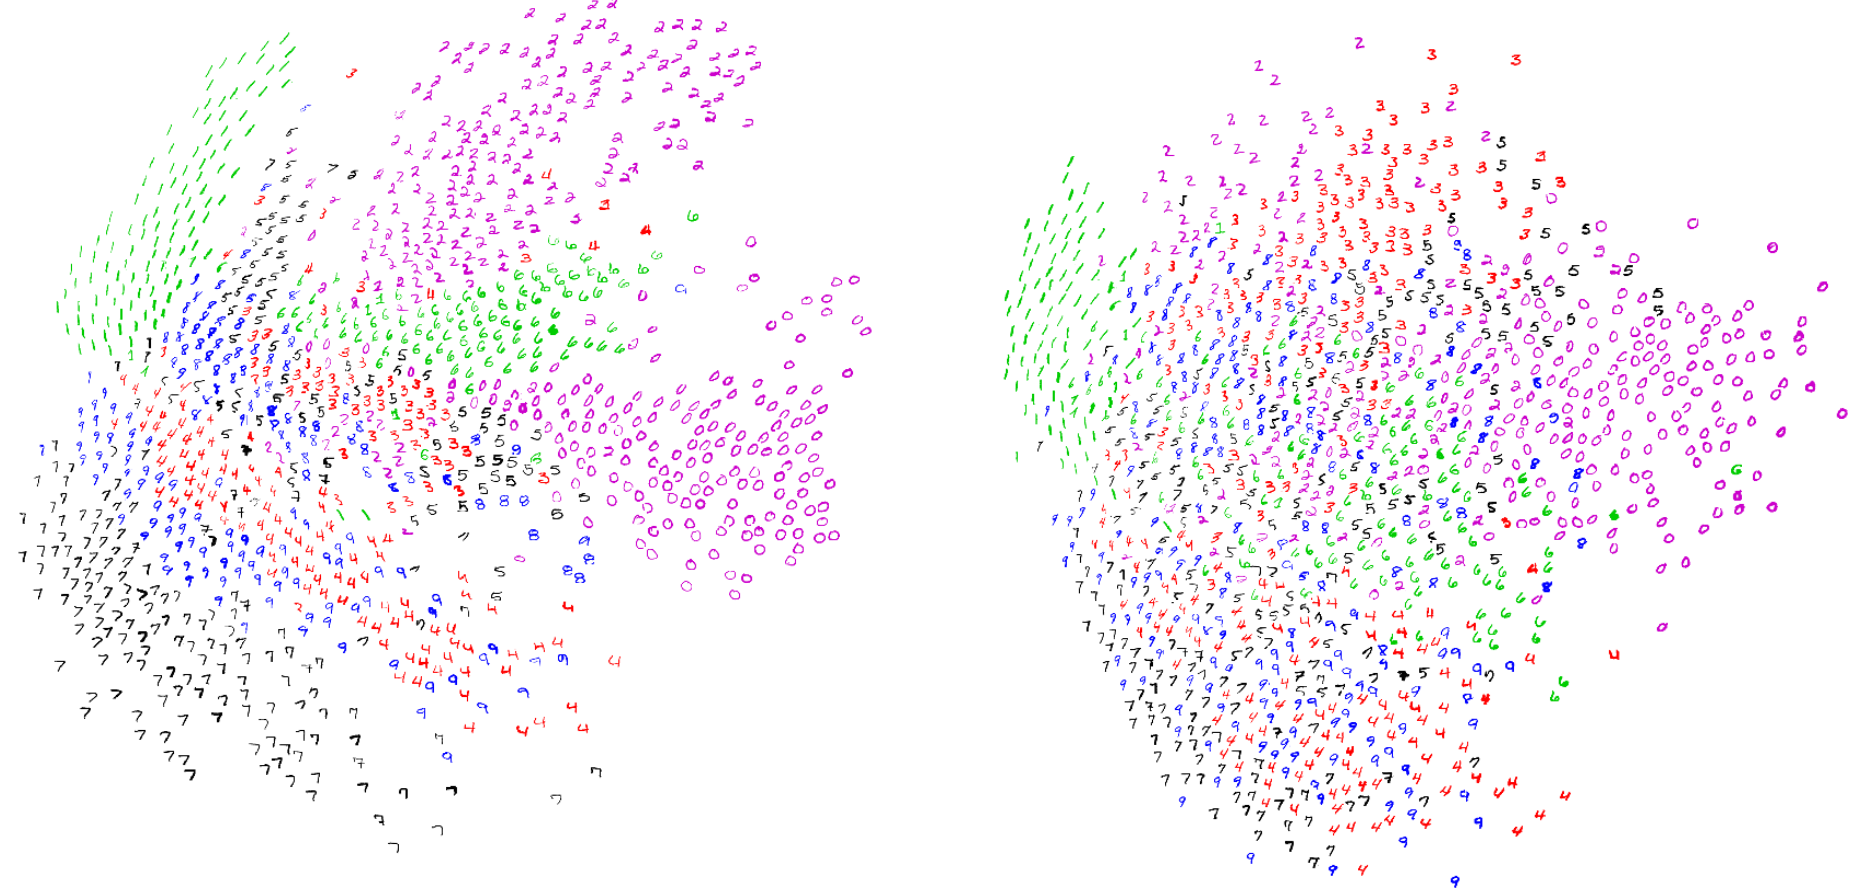
\includegraphics[width=\linewidth]{abbildungen/mnistvisualize.png}
  \caption{Visualizations of encoded two-dimensional Vector from the MNIST dataset: The encoded vectors created by an autoencoder (left) show better separated groups of each classes than those created by using principle component analysis method (right).}
  \label{fig:mnistvisualize} 
\end{figure}

\subparagraph*{Extracting Features}
Being able to compress data into lower-dimensional, the autoencoders know how to find the essential features of the data. By using features discovered by the autoencoders, the results of the classifier has been improved as shown by \cite{autoencoderDenoise}.


So far, we discuss the idea of the artificial neural networks, their structures, the training method and its problem in general. Now, we will study a specific kind of problem in machine learning when the training data and the test data are from different distribution. In this situation, the network must be able to learn to counter the change in the distribution and to generalize from one set to another. We have to introduce domain adaptation to the problem. 

Up to this point, the idea of neural networks and their basic functions of learning and making predictions were introduced. As a network learns, it adjusts the parameters in a way that it can make the most accurate prediction according to the training data. A common method to do this despite several layers and millions of neurons is to use backpropagation and gradient descent method. Backpropagation traces back into the hidden layers to find their relations to the output while gradient descent indicates the direction of the adjustment resulting in a decrease of the errors of the network. In the experiments, the network used also implement these methods with momentum as an optimizer for the gradient descent step. 

Since traditional learning methods only learn from the training data without expecting different distribution in the new data it should perform its task on,  it will perform badly if such a difference in the data distribution exists. To counter this problem and train the machine to generalize from one domain to another, domain adaptation method is introduced. 

In this thesis, we investigate a specific case in domain adaptation in which the source domain consists of mixture of data from different domains building up a complete set of all competing classes and the target domain the unseen class-domain combination. For this task, we chose a neural network specialized in learning with domain adaptation. The next section will first introduce the problem of domain adaptation and its special case of domain mixture scenario.